\documentclass[12pt,a4paper]{article}
\usepackage[14pt]{extsizes}
\usepackage[french]{babel}
\usepackage[utf8]{inputenc}
\usepackage[T1]{fontenc}
\usepackage{wrapfig}
\usepackage{amsmath}
\usepackage{array}
\usepackage{graphicx}
\usepackage{tikz}

\title{}
\author{}
\date{}

\newcommand{\subtitle}{Rapport de projet\\Soutenance IV}

\begin{document}
	\begin{titlepage}
		\begin{center}
			\vspace{8cm}
			
\includegraphics[width=15cm]{images/spacesymphonia.png}
			\vspace{0.5cm}
			\par \LARGE{\textbf{\subtitle}}
			\vspace{1cm}
			\par \large{\textsf{
				Emmanuel `Green` \bsc{Guet} \\
				Antoine `Nervous` \bsc{Vallée} \\
				Antoine `serialk` \bsc{Pietri}}}
			\vspace{2cm}
			\par \large{\textsf{Projet d'InfoSup --- EPITA}}
		\end{center}
	\end{titlepage}
	
	\newpage
	Cette page est laissée intentionnellement vide.	
	
	\newpage
	\par \textbf{Avertissement}
	\vspace{2cm}
	\par Ce rapport est vendu avec les éléments suivants :
	\begin{itemize}
		\item Un DVD-ROM d'installation avec une jaquette super bien faite ;
		\item Un manuel d'utilisation ;
		\item Un manuel d'installation ;
		\item Un plan de soutenance\footnote{Pour ne pas se perdre dans la soutenance.}.
	\end{itemize}
	\vspace{1cm}
	\par Ces éléments ne peuvent être vendus séparément.
	\par Si ce rapport vous a été vendu
	sans un de ces éléments, contactez au plus vite le service de répression des fraudes
	au 04 04 13 37 42. 
	
	\newpage
	\setcounter{tocdepth}{3}
	\tableofcontents
	
	\newpage
	\pagestyle{headings}
	
	\section{Introduction}
		\par
		L'objectif de ce rapport de projet est de présenter l'ensemble du travail
		accompli durant l'année par l'équipe \texttt{TEUH TEUH TEUH} sur le projet de jeu \emph{Space Symphonia}.
		\par La présentation de ce travail se fera de manière chronologique, et chacune des parties sera détaillée pour vous présenter le contenu ajouté progressivement au fil des soutenances. S'ensuivra ensuite un récit de la réalisation et des difficultés que nous avons pu rencontrer au cours du développement de ce projet, puis un bref récapitulatif sur la correspondance du résultat final par rapport à nos attentes.
		\vspace{2cm}
		\par \emph{Oh, you should have seen it! That old planet... The second sun would rise in the south, and the mountains would shine. The leaves on the trees were silver, when they caught the light, every morning it looked like a forest on fire. When the autumn came, a brilliant glow though the branches\ldots}
	
	\newpage
	\section{Rappels sur le principe du jeu}
		\par Notre projet était de réaliser un jeu, plus précisément un Shoot Them Up dans l'espace.
Le joueur contrôle un vaisseau et doit tuer le plus de vaisseaux ennemis possible sans mourir.
\par Nous avons développé quatre différents modes :
\begin{itemize}
	\item Le mode \textbf{campagne}, dans lequel le joueur progresse au cours des niveaux et rencontre des boss en difficulté progressive.
	\item Le mode \textbf{extrême}, un seul niveau dans lequel tous les boss sont rassemblés que vous devez finir d'une traite.
	\item Le mode \textbf{niveaux personnalisés}, où il est possible de choisir des niveaux créés avec l'éditeur de niveau intégré
	\item Le mode libre, dans lequel le joueur choisit une musique, l'analyse, et génère un niveau en fonction de son rythme et de sa puissance.
\end{itemize}

\par Nous avons avons progressivement ajouté de plus en plus de contenu (boss, ennemis, missiles, bonus\ldots), que nous vous laissons découvrir dans ce rapport.
	
	
	\newpage
	\section{Frise chronologique de l'avancement}
		\begin{tikzpicture}
	\draw[gray,->] (0,0) coordinate (tl1start) -- ++(0,-500pt) coordinate
	(tl1end);
	\draw[gray,->] (tl1start)++(100pt,0) coordinate (tl2start)-- +
	+(0,-500pt) coordinate (tl2end);
	\path (tl1start) --
		node[left,pos=0.25] {\textbf{1e soutenance}}
		node[left,pos=0.50] {\textbf{2e soutenance}}
		node[left,pos=0.75] {\textbf{3e soutenance}}
		node[left,pos=0.99] {\textbf{4e soutenance}}
		node[right,pos=0.25] {\small{\textbf{06/01/12}}}
		node[right,pos=0.50] {\small{\textbf{02/03/12}}}
		node[right,pos=0.75] {\small{\textbf{04/05/12}}}
		node[right,pos=1] {\small{\textbf{18/06/12}}}
	(tl1end);
	\path (tl2start) --
	node[left,pos=0.01] {\scriptsize{23/09/11}}
	node[right,pos=0.01] {\scriptsize{Premiers déplacements}}
	node[left,pos=0.04] {\scriptsize{26/09/11}}
	node[right,pos=0.04] {\scriptsize{Collisions \& missiles}}
	node[left,pos=0.08] {\scriptsize{30/09/11}}
	node[right,pos=0.08] {\scriptsize{Gestion des niveaux}}
	node[left,pos=0.11] {\scriptsize{13/10/11}}
	node[right,pos=0.11] {\scriptsize{Moteur à particules}}
	node[left,pos=0.16] {\scriptsize{5/12/11}}
	node[right,pos=0.16] {\scriptsize{Gestion des scores}}
	node[left,pos=0.19] {\scriptsize{10/12/11}}
	node[right,pos=0.19] {\scriptsize{Implémentation de FMOD}}
	node[left,pos=0.22] {\scriptsize{20/12/11}}
	node[right,pos=0.22] {\scriptsize{Affichage du spectre sonore}}
	%Soutenance 1
	node[left,pos=0.30] {\scriptsize{07/02/12}}
	node[right,pos=0.30] {\scriptsize{Amélioration de l'interface}}
	node[left,pos=0.33] {\scriptsize{10/02/12}}
	node[right,pos=0.33] {\scriptsize{Calcul de l'énergie musicale}}
	node[left,pos=0.36] {\scriptsize{12/02/12}}
	node[right,pos=0.36] {\scriptsize{Modification de la vitesse du jeu selon la musique}}
	node[left,pos=0.39] {\scriptsize{19/02/12}}
	node[right,pos=0.39] {\scriptsize{Ajout de nouveaux ennemis}}
	node[left,pos=0.42] {\scriptsize{25/02/12}}
	node[right,pos=0.42] {\scriptsize{Implémentation du premier boss}}
	node[left,pos=0.45] {\scriptsize{26/02/12}}
	node[right,pos=0.45] {\scriptsize{Changement de l'HUD, amélioration des particules}}
	node[left,pos=0.48] {\scriptsize{27/02/12}}
	node[right,pos=0.48] {\scriptsize{Modulation des particules selon la musique}}
	%Soutenance 2
	node[left,pos=0.53] {\scriptsize{01/04/12}}
	node[right,pos=0.53] {\scriptsize{Implémentation de la détection de battements}}
	node[left,pos=0.55] {\scriptsize{02/04/12}}
	node[right,pos=0.55] {\scriptsize{Changement de l'interface}}
	node[left,pos=0.57] {\scriptsize{03/04/12}}
	node[right,pos=0.57] {\scriptsize{Implémentation du mode libre}}
	node[left,pos=0.59] {\scriptsize{04/04/12}}
	node[right,pos=0.59] {\scriptsize{Implémentation des trous noirs}}
	node[left,pos=0.61] {\scriptsize{05/04/12}}
	node[right,pos=0.61] {\scriptsize{Détection du tempo}}
	node[left,pos=0.63] {\scriptsize{08/04/12}}
	node[right,pos=0.63] {\scriptsize{Calcul du hash MD5 de la musique comme seed du PRNG}}
	node[left,pos=0.65] {\scriptsize{28/04/12}}
	node[right,pos=0.65] {\scriptsize{Nouvelles armes}}
	node[left,pos=0.67] {\scriptsize{01/05/12}}
	node[right,pos=0.67] {\scriptsize{Ajout du deuxième boss}}
	node[left,pos=0.69] {\scriptsize{02/05/12}}
	node[right,pos=0.69] {\scriptsize{Ajout du troisième boss}}
	node[left,pos=0.71] {\scriptsize{03/05/12}}
	node[right,pos=0.71] {\scriptsize{Nouveaux ennemis et bonus, nouveau missile à particules}}
	node[left,pos=0.73] {\scriptsize{03/05/12}}
	node[right,pos=0.73] {\scriptsize{Création de l'éditeur de niveau}}
	%Soutenance 3
	node[left,pos=0.78] {\scriptsize{22/05/12}}
	node[right,pos=0.78] {\scriptsize{Ajout d'un nouvel ennemi}}
	node[left,pos=0.80] {\scriptsize{10/06/12}}
	node[right,pos=0.80] {\scriptsize{Ajout de deux nouveaux ennemis}}
	node[left,pos=0.82] {\scriptsize{12/06/12}}
	node[right,pos=0.82] {\scriptsize{Progression de la musique dans le mode libre}}
	node[left,pos=0.84] {\scriptsize{13/06/12}}
	node[right,pos=0.84] {\scriptsize{Ajout de l'importation dans l'éditeur}}
	node[left,pos=0.86] {\scriptsize{15/06/12}}
	node[right,pos=0.86] {\scriptsize{Lecture des métadonnées des fichiers audio}}
	node[left,pos=0.88] {\scriptsize{15/06/12}}
	node[right,pos=0.88] {\scriptsize{Ajout des boss 4 et 5}}
	node[left,pos=0.90] {\scriptsize{13/06/12}}
	node[right,pos=0.90] {\scriptsize{Ajout de l'exportation dans l'éditeur}}
	node[left,pos=0.92] {\scriptsize{16/06/12}}
	node[right,pos=0.92] {\scriptsize{Nom du joueur dans les scores}}
	node[left,pos=0.94] {\scriptsize{16/06/12}}
	node[right,pos=0.94] {\scriptsize{Possibilité d'accélérer les musiques}}
	(tl2end);
\end{tikzpicture}

\par (Ceci n'est pas (seulement) un prétexte pour jouer avec tikzfig).
	
	\newpage
	\section{Présentation globale du contenu}
		\subsection{Vaisseaux}
			\par Le membre du groupe responsable de cette partie était Emmanuel Guet.

Dans un jeu de type Shoot'Em, il est évident que les ennemis font partie intégrante du jeu.
C'est pourquoi le travail les concernant a été conséquent, et il en résulte une flopée d'ennemis, dont le rôle diffère réellement d'un ennemi à un autre. Cette partie est là pour tenter de les expliquer au mieux, en donnant quelques statistiques les concernant.

		\begin{itemize}
			\item[$\bullet$ Drone]
				\par~
				\begin{itemize}
					\item Vie : 20
					\item Dommages en cas de collision : Faibles
					\item Vitesse : Rapide
					\item Aptitude : Blaster
					\item Dangerosité : 5%
					\item Rôle : Il s'agit de l'ennemi le moins dangereux, mais aussi de l'ennemi le plus présent. Il ne dispose d'aucune capacité spécifique, et son attaque, un Aptitude au Blaster, n'inflige que peu de dégâts, c'est pourquoi sa dangerosité est si basse.
				\end{itemize}

\includegraphics[width=11cm]{images/vaisseaux/drone.png}
				\par~
			\item[$\bullet$ Double Shooter]
				\par~
				\begin{itemize}
					\item Vie : 40
					\item Dommages en cas de collision : Faibles
					\item Vitesse : Rapide
					\item Aptitude : Blaster ($\times2$)
					\item Dangerosité : 10%
					\item Rôle : Une évolution du Drone. En conséquence, la dangerosité reste basse, toutefois se faire toucher par plusieurs rafales d'affilée implique des dégâts conséquents.
				\end{itemize}
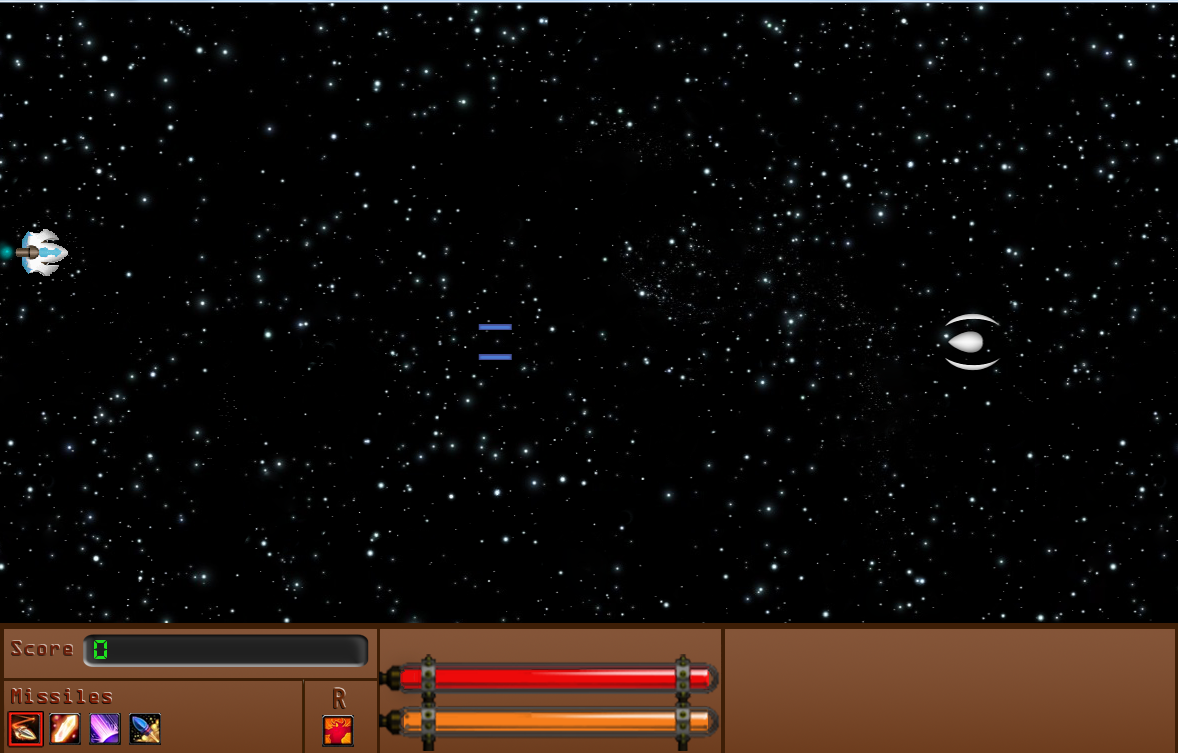
\includegraphics[width=11cm]{images/vaisseaux/doubleshooter.png}
			\item[$\bullet$ Blasterer]
				\par~
				\begin{itemize}
					\item Vie : 50
					\item Dommages en cas de collision : Faibles
					\item Vitesse : Lente
					\item Aptitude : Énergie filée
					\item Dangerosité : 15%
					\item Role : L'ennemi le plus résistant à l'heure actuelle. Il avance lentement, Aptitude à cadence lente avec une arme infligeant des dégâts importants. Il est vital de ne pas subir plusieurs fois de l'énergie filée ...
				\end{itemize}
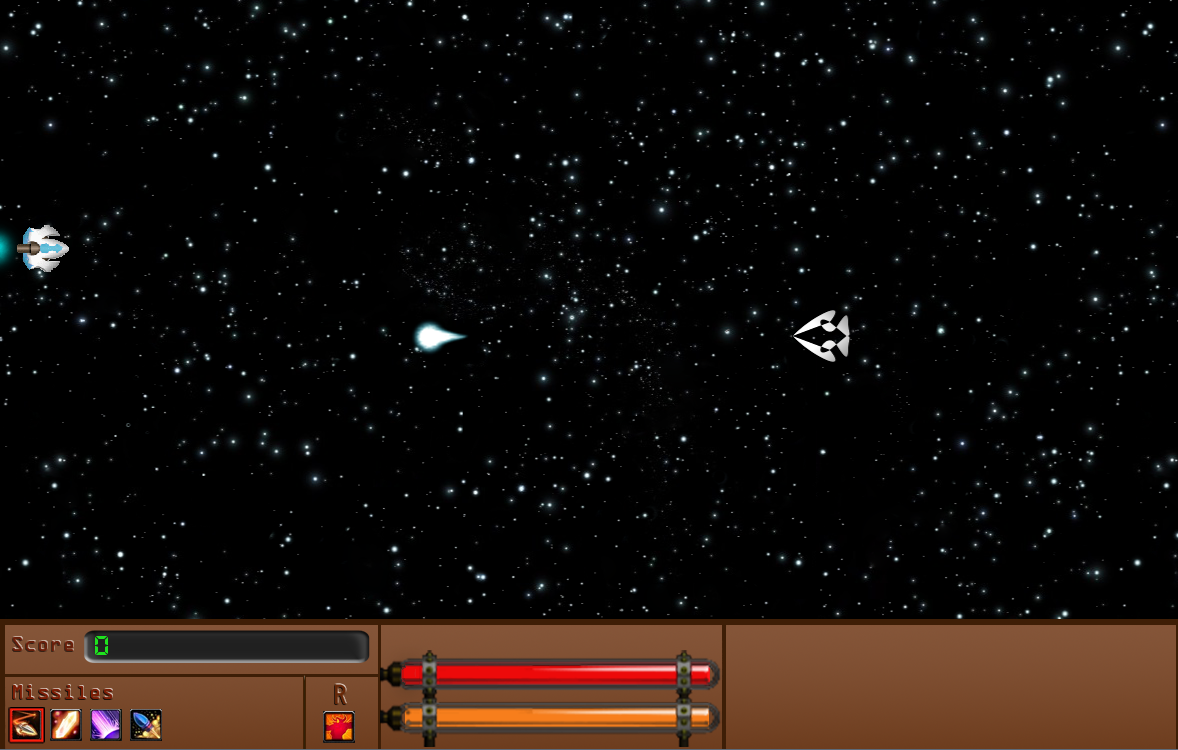
\includegraphics[width=11cm]{images/vaisseaux/blasterer.png}
				\par~
			\item[$\bullet$ Kamikaze]
				\par~
				\begin{itemize}			
					\item Vie : 5
					\item Dommages en cas de collision : Très élevés
					\item Vitesse : Très rapide
					\item Aptitude : Aucun
					\item Dangerosité : 25%
					\item Rôle : Un ennemi très rapide et qui inflige d'énorme dégâts à l'impacte. Tel un kamikaze, il cherche à s'encastrer contre le vaisseau du joueur, lui enlevant ainsi 1/5e de sa vie. Il devient ainsi un ennemi dont le potentiel dangereux commence à devenir important.
				\end{itemize}
				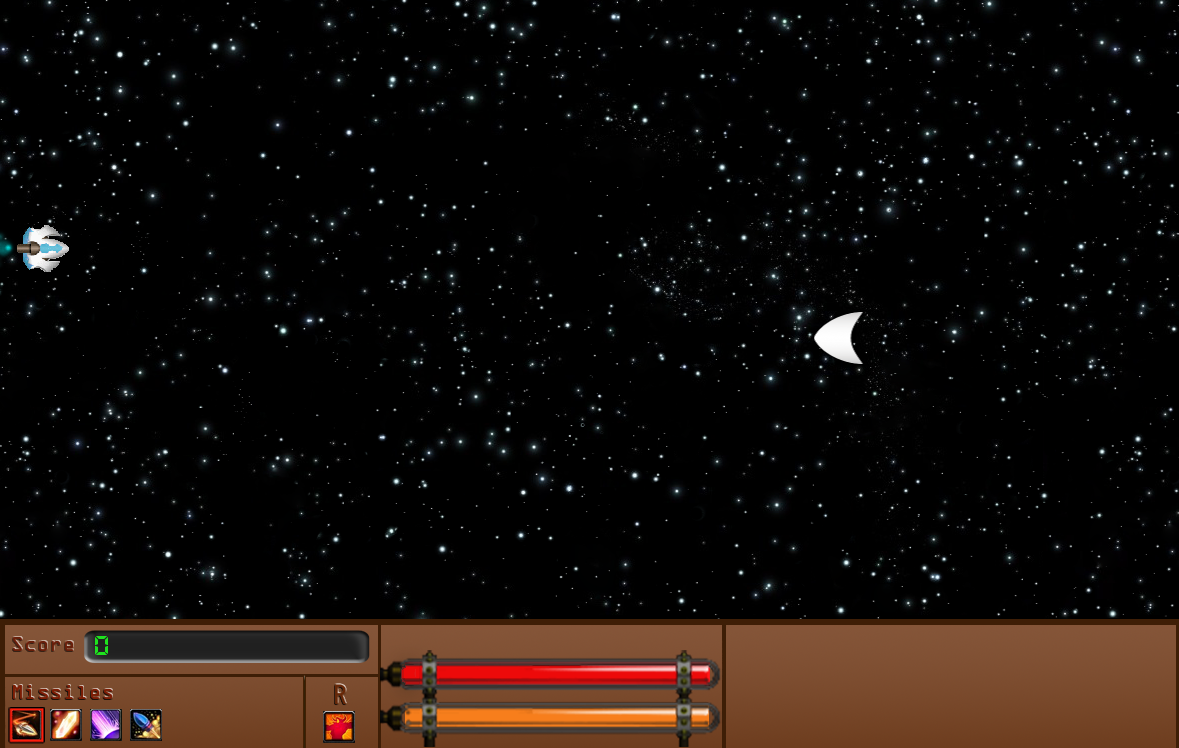
\includegraphics[width=11cm]{images/vaisseaux/kamikaze.png}
				\par~
					\item[$\bullet$ Zebra]
				\par~
				\begin{itemize}
					\item Vie : 5
					\item Dommages en cas de collision : Faibles
					\item Vitesse : Moyenne
					\item Aptitude : Aucun
					\item Dangerosité : 10%
					\item Rôle : Il s'agit d'un ennemi qui bouge de haut en bas dans le niveau. Il est là pour obliger le joueur à augmenter sa vigilance, mais reste un ennemi peu dangereux. Attention toutefois s'il en apparait plusieurs, ils peuvent rapidement devenir dangereux.
				\end{itemize}
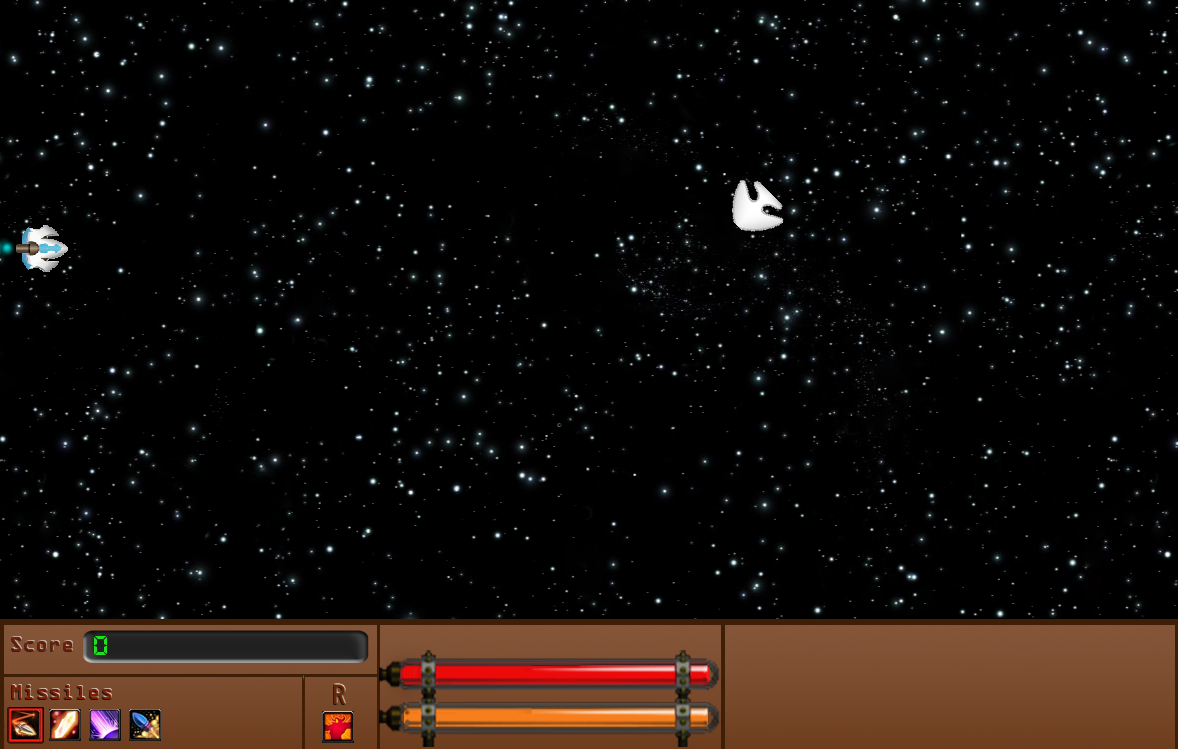
\includegraphics[width=11cm]{images/vaisseaux/zebra.png}
				\par~
				\item[$\bullet$ Battle Cruiser]
				\par~
				\begin{itemize}
					\item Vie : 50
					\item Dommages en cas de collision : Faibles
					\item Vitesse : Moyenne
					\item Aptitude : Chargement du laser - Laser
					\item Dangerosité : 50%
					\item Role : Le premier ennemi réellement dangereux. Il va charger un laser boosté à l'ambodium, une technologie alien, qui permet d'infliger des dégâts incroyablement élevés. De plus, étant invincibles pendant ce chargement, une fois commencé, rien ne peut les arrêter. Faites-attention !
				\end{itemize}
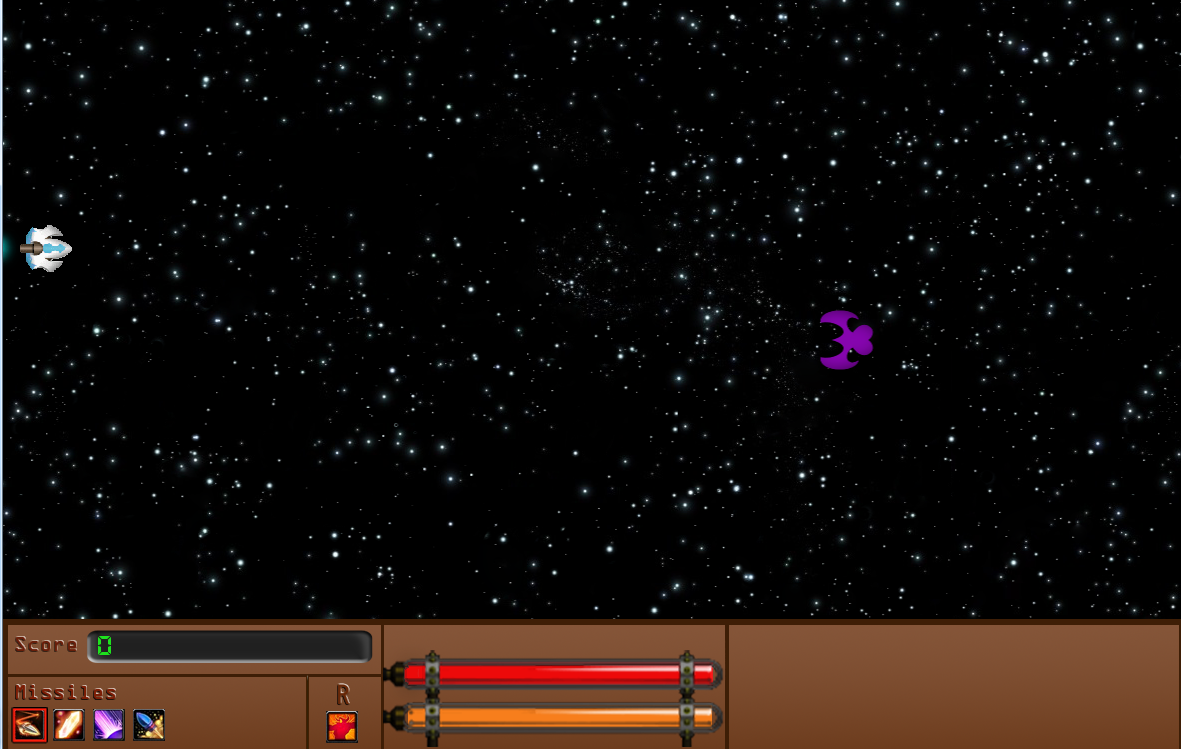
\includegraphics[width=11cm]{images/vaisseaux/bc_load.png}
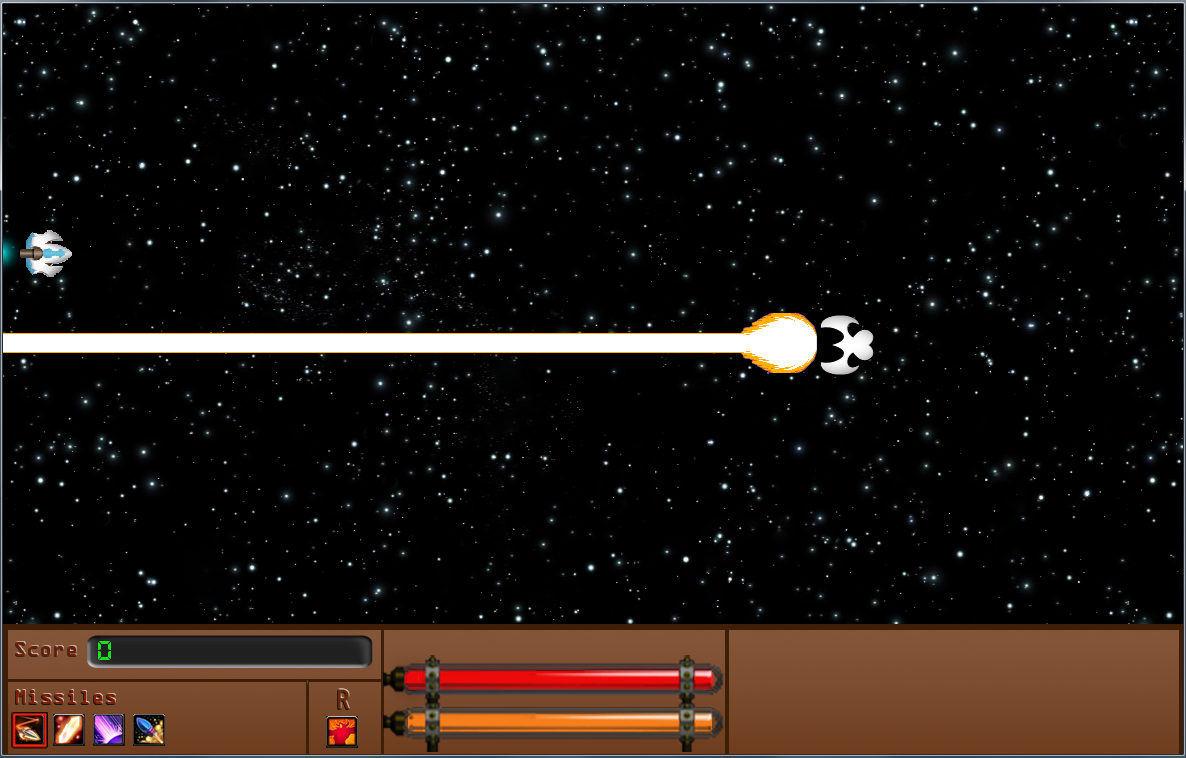
\includegraphics[width=11cm]{images/vaisseaux/bc_fire.png}

				\par~
				\item[$\bullet$ Targeter]
				\par~
				\begin{itemize}
					\item Vie : 50
					\item Dommages en cas de collision : Faibles
					\item Vitesse : Moyenne
					\item Aptitude : Boule d'énergie autoguidée
					\item Dangerosité : 45%
					\item Rôle : Le Targeter a la capacité de pouvoir tirer une boule d'énergie autoguidée, qui va donc suivre le joueur. Le seul moyen de s'en séparer et de s'en rapprocher suffisamment. Adrénaline garantie !
				\end{itemize}

\includegraphics[width=11cm]{images/vaisseaux/targeter.png}
				\par~
				\item[$\bullet$ Support]
				\par~
				\begin{itemize}
					\item Vie : 50
					\item Dommages en cas de collision : Faibles
					\item Vitesse : Très rapide mais s'arrête au milieu de l'écran
					\item Aptitude : Aura généreuse
					\item Dangerosité : 70%
					\item Rôle : Cet ennemi est sans aucun doute le plus dangereux. Et pourtant, il ne possède aucune capacité offensive. Il va s'installer au milieu de l'écran et déployer son aura généreuse, qui divise tous les dégâts infligés par le joueur par 4. La taille de l'aura augmente au fur et à mesure que le support est présent sur le terrain. Attention à ne pas le laisser en vie trop longtemps sous peine de défaite obligatoire !
				\end{itemize}
				\begin{center}
					\par 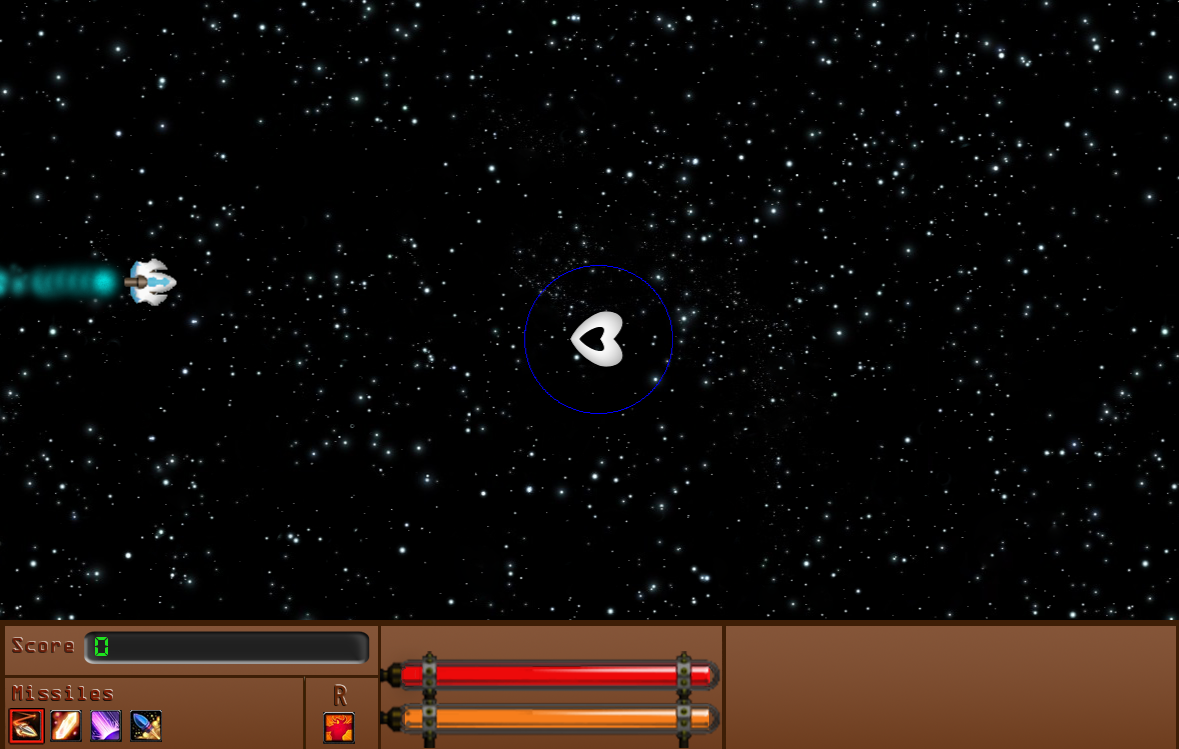
\includegraphics[width=11cm]{images/vaisseaux/support_little.png}
					\par 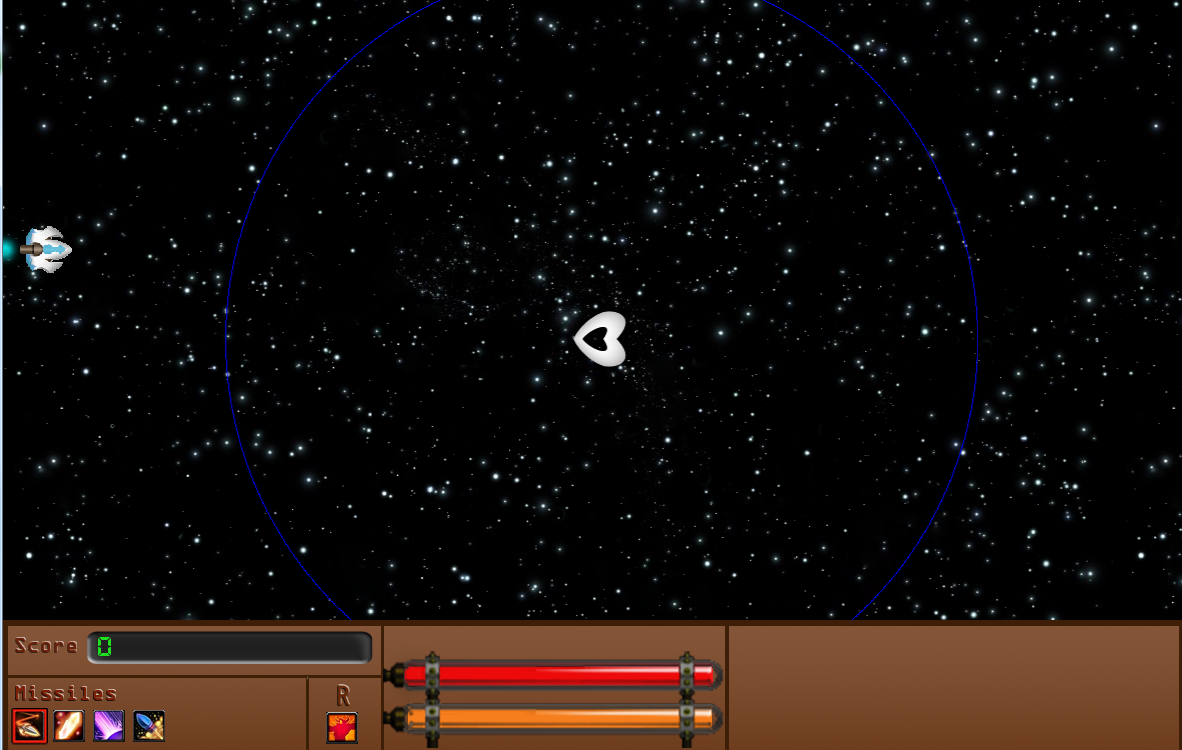
\includegraphics[width=11cm]{images/vaisseaux/support_huge.png}
				\end{center}

				\par~
		\end{itemize}
		\subsection{Armes, bonus et améliorations}
			\par Le membre du groupe responsable de cette partie était Emmanuel Guet.
		\subsection{Boss, mode extrême}
			\par Le membre du groupe responsable de cette partie était Antoine Vallée.

\par Dans un Shoot Them All, l'intelligence artificielle n'est pas vraiment présente dans la plupart des phases du jeu: Les ennemis de base n'effectuent que de simple actions qui se révèlent être toujours les même. Toutefois, il nous paraissait important de travailler sur cet aspect des jeux vidéos, qui nous parait primordiale.
\par C'est pourquoi nous avons très vite décidé que des boss seraient présents dans le jeu, et qu'ils traduiraient concrètement notre travail sur l'intelligence artificielle. Nous nous étions fixé un objectif de 5 boss, et nous y sommes arrivé, sans trop de mal d'ailleurs. Seul un membre du projet aura eu à se concentrer sur cette tâche.
\par Pour développer nos boss, nous nous sommes inspirés de jeux récents ayant faits leur succès dans l'intelligence artificielle, en nous basant sur un système largement répandu, mais aussi très efficace, de phases. En effet, chaque combat contre un boss est divisé en plusieurs phases, qui se déclenchent en fonction de la vie du boss ou du temps écoulé. Ce système de phase est primordiale car il apporte une dynamisme au combat qu'aucun autre système ne saurait apporter. Il permet de ne pas geler le boss à une seule stratégie, qu'il appliquera tout le long du combat, mais de lui donner la possibilité d'appliquer plus de 3 stratégies différentes en fonction des situations.
\par Avec ces changements de stratégies en plein combat, le joueur se retrouve à devoir constamment changer de tactique pour ne pas mourir et pour éliminer le boss. Graphiquement cela demande un travail colossal en plus (nombreux missiles par boss, météorites etc..), mais ça en vaut la peine.
\par Ainsi, nous avons développé ces boss au fur et à mesure de l'année, nous en avons présenté un à la première soutenance, qui fut le plus long à développer puisqu'il fallait créer toute la structure même des boss, puis nous en avons présenté trois en troisième soutenance, pour finir avec un total de cinq sur la version finale du projet.

\par Photo boss1   Nom: Spaceship X-42
               Tactique: En phase 1, le boss va tirer des salves de missiles tout en se déplaçant de haut en bas. Une fois entré en phase 2, il va se déplacer beaucoup plus vite et le joueur devra vite lui faire perdre de la vie. La phase 3 est elle, bien plus intéressante: Le boss devient invincible, entouré d'un bouclier bleu. Il tire sans s'arrêter, puis perd son bouclier quelques secondes. C'est à ce moment là que le joueur doit le toucher, tout en évitant ses missiles dévastateurs.
			   
Photo boss2   Nom: Metal'Krisboul
				Tactique: En phase 1, le boss va seulement se déplacer de haut en bas sans tirer. Toutefois en phase 2 une pluie de météores va s'abattre sur le joueur, qui va devoir les éviter tout en continuant de tirer sur le boss. Passée cette pluie, le boss va se mettre à tirer des salves de trois missiles, dont deux en diagonales qui feront perdre énormément de vie au joueur. Bonne chance !
				
Photos boss3  Nom: Tie supressor
				Tactique: En première phase, le boss va tirer des salves de missiles. Puis, une fois en danger, il va se replier et appeler en renfort de nombreux ennemis. Le joueur devra les détruire, et affaiblir le boss une fois réapparu. Si il ne le tue pas assez vite, d'autres renforts vont arriver, et il se retrouvera vite submergé.
				
Photos boss45 Nom: The All-Seeing Eye
				Tactique: Ce boss peut paraitre anodin à première vue: Un simple oeil. Mais détrompez vous, malgré une phase 1 relativement simple (un simple tir de missile), la suite va être très corsée. En effet, le boss va se téléporter dans tout l'écran, créant autour de lui un énorme cercle que le joueur devra absolument éviter. Ce dernier n'aura qu'une seconde pour réagir et se déplacer avant l'apparition du cercle, tout en ayant sa vitesse extrêmement réduite. Il devra aussi faire preuve de rapidité et tirer sur le boss une fois 4 téléportations effectuées: C'est à ce moment là qu'il ne sera plus intouchable.
				
Photo boss5   Nom: NathalisBoulax
				Tactique: Surprise.
		\subsection{Obstacles}
			\par Le membre en charge de cette partie était Antoine Pietri.

\par Les seuls obstacles que nous avons implémenté dans le jeu sont les trous noirs.
\par Nous nous sommes peu à peu rendu compte que ces obstacles encombraient trop le jeu et n'avaient
que peu d'utilité, c'est pourquoi nous avons décidé de ne pas en rajouter.
\par Les trous noirs sont des objets assez complexes puisqu'ils attirent le joueur en leurs centres en les faisant
tourner, ce qui a nécessité une bonne utilisation de nos connaissances en cinématique.

\begin{center}
	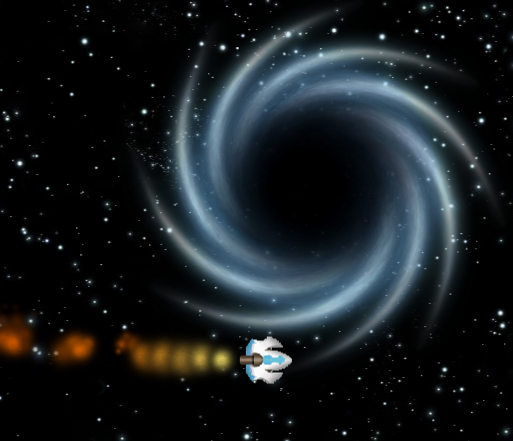
\includegraphics[width=260pt]{images/blackhole.png}
\end{center}

\par Leur but est donc d'attirer puis de bloquer le joueur en leurs centres. Pour cela nous procédons ainsi :
\begin{itemize}
	\item On commence par passer en coordonnées polaires dans un repère centré sur l'obstacle :
	$$ X_a = X_{vaisseau} - X_{obstacle} $$
	$$ Y_a = Y_{vaisseau} - Y_{obstacle} $$
	$$ R = \sqrt{X_a^2 + Y_a^2} $$
	$$ \theta = arctan(Y_a / X_a) $$
	
	\item On modifie $r$ et $\theta$ pour faire l'effet d'une spirale, on retourne en cartésien, puis on retourne dans le repère d'origine :
	$$X_{vaisseau} = (r - \Delta t \frac{G}{r^2}) \times cos(\theta - \Delta t \frac{\phi}{r^2}) + X_{obstacle}$$
	$$Y_{vaisseau} = (r - \Delta t \frac{G}{r^2}) \times sin(\theta - \Delta t \frac{\phi}{r^2}) + Y_{obstacle}$$
	avec $\phi$ et $G$ constantes (dans le jeu respectivement 1000 et 30), et $\Delta t$ le temps écoulé en secondes.
\end{itemize}
		\subsection{Éditeur de niveau}
			subsection{Editeur de niveau}
\par Notre jeu �tant un shoot them all, il nous a paru �vident que nous aurions besoin d'un �diteur de niveau, et ce, d�s le d�part. Ce dernier permettrait aux joueurs de renouveller eux m�me le contenu.
\par Le d�veloppeur de l'�diteur a d�but� pour la soutenance 3, le d�but fut laborieux: La prise en main des winforms, le design de l'�diteur.. Mais une fois le tout bien lanc�, le d�veloppement �tait bien partit. Toutefois, d�velopper l'�diteur de niveau a �t� une rude t�che. L'�criture des niveaux repose sur les streamwriter, les buffers.. bel apprentissage. Si ce n'est qu'il fallait pouvoir rendre possible l'�dition d'un vaisseau d�j� plac�.
\par Le premier probl�me se trouver l�, il fallait pouvoir d�velopper un syst�me permettant de se d�placer tr�s aisement dans un fichier de niveau, ce ne fut pas simple, mais d'autres �preuves firent leurs apparitions. Tout d'abord, g�rer le temps. En effet, il est impossible d'afficher un niveau entier dans l'�diteur, nous avons donc fractionn� ces niveaux en "pages" de 3200ms, puis en colonnes de 400ms. Toutefois, si nous voulions rendre possible l'�dition de page pr�c�demment remplies, il fallait pouvoir lire un fichier de niveau et l'interpreter convenablement.
\par La plus grosse difficult�e de l'�diteur fut ici: L'interpretation d'un fichier de niveau. Replacer au bon endroit les vaisseaux, dans la bonne colonne, avec l'image correspondante. Cela n'�tait pas encore possible � la soutenance 3, mais �a l'est pour la version finale.
\par L'interpretation nous permet aussi donc d'importer des fichiers de niveaux: Chaque joueur pourra donc modifier n'importe quel niveau du jeu, qu'il a cr��, ou qu'un ami lui a donn�. L'�diteur lui permet de tout modifier. L'exportation du niveau du joueur �tait aussi bien s�r n�cessaire, dans le but de sauvegarder ce dernier, et de jouer sur le niveau.
\par Ainsi, l'�diteur est donc tr�s complet: Il regroupe tout le contenu du jeu, il est possible d'importer, d'exporter des niveaux, et donc de les partager avec vos amis ! M�me si graphiquement il semble basique, notre �diteur est donc un outils tr�s puissant, qui nous fut d'ailleurs tr�s utile pour construire nos niveaux dans le mode Campagne.
Evolution de l'�diteur de niveau:
Soutenance 3:
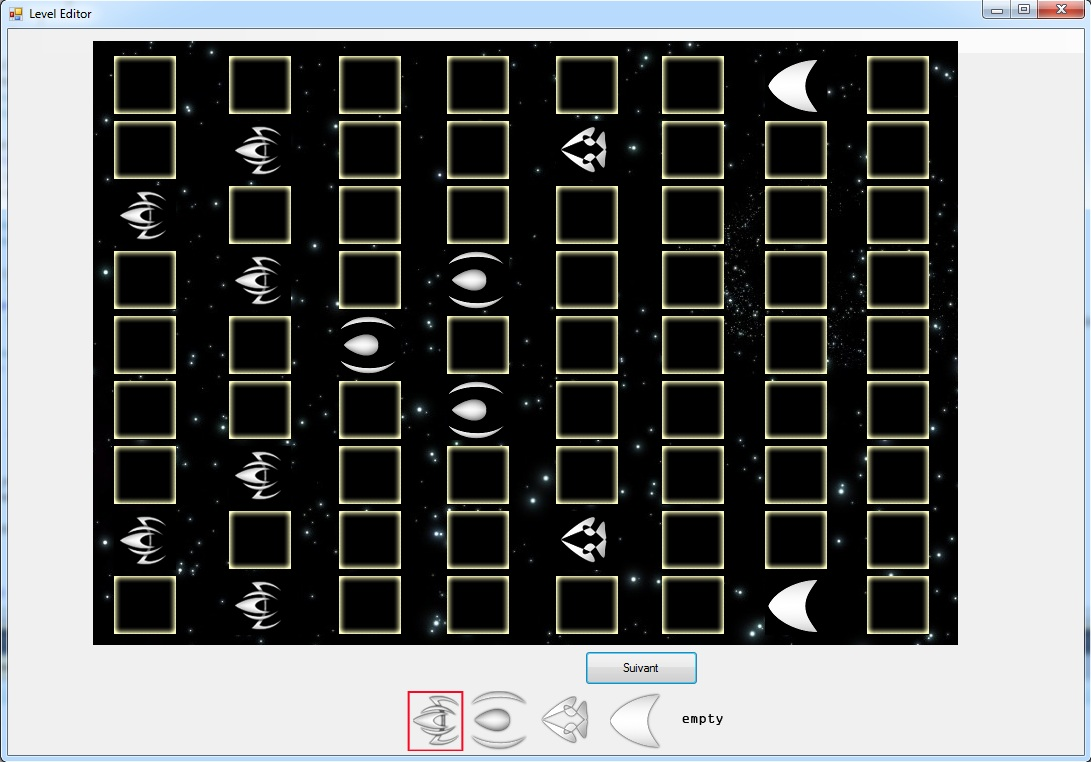
\includegraphics{images/leveleditor2.jpg}
Version finale:
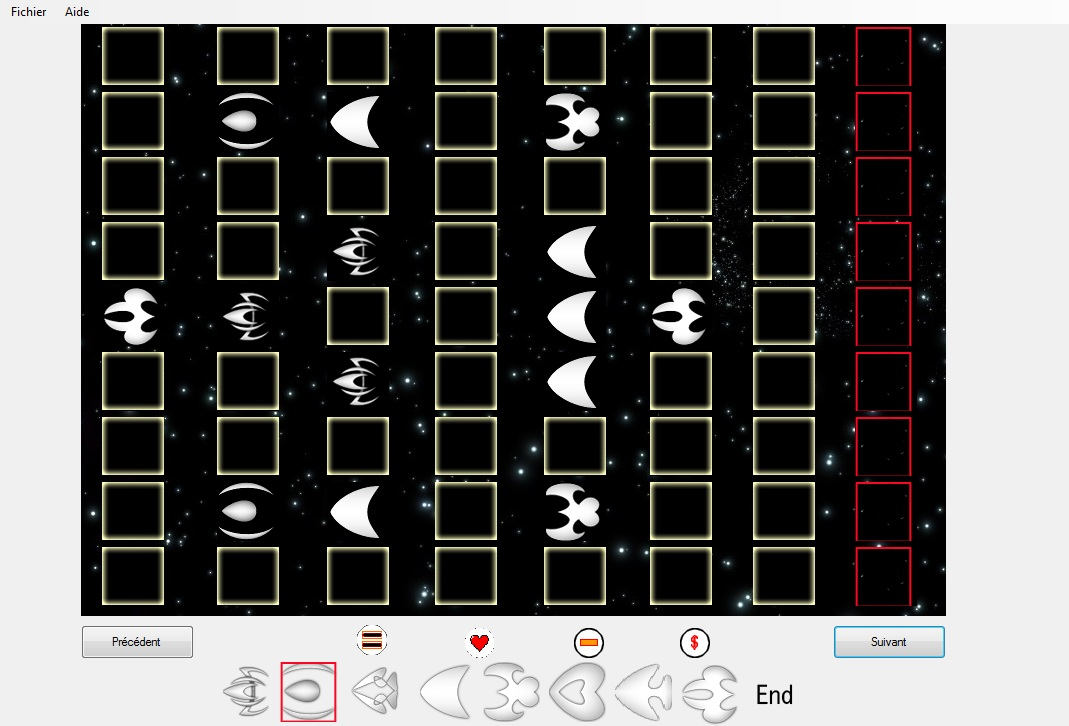
\includegraphics{images/leveleditor.jpg}
		\subsection{Analyse sonore et mode libre}
			\par Le membre du groupe en charge de cette partie était Antoine Pietri.
\vspace{1cm}
\par Dès le début du projet, nous souhaitions donner à l'analyse de la musique un rôle central dans notre jeu.
Nous avons, en plusieurs étapes, progressé vers un jeu (et ce en particulier dans le mode libre) où la musique
dynamise entièrement le jeu.

\subsubsection{Utilisation de FMOD}

La première chose dont nous avions besoin pour débuter dans l'analyse de la musique était une bibliothèque
qui nous permettait d'accéder aux données d'onde. Nous avons choisi FMOD, qui fournit un wrapper en C\#

\subsubsection{Détection de battements : algorithme de base}

\par Pour implémenter le mode Libre, nous avions besoin de détecter les \emph{battements} de la musique choisie par l'utilisateur, et nous avons effectué beaucoup de recherches sur la détection de battements.

\par Pour la troisième soutenance, nous vous avions présenté une version de l'algorithme de détection de battements déjà fonctionnelle, qui a cependant été optimisée depuis.
	
\par Simuler un phénomène physique qui obéit à des équations mathématiques connues est, avec un certain nombre d'approximations, toujours faisable. Mais les concepts plus abstraits, comme les sensations, qui n'obéissent à aucune loi sont souvent bien plus complexes à capturer dans un programme. Le ressenti des battements lors de l'écoute d'une musique est par exemple un phénomène naturel inné chez l'homme. Cependant il existe un certain nombre d'algorithmes qui essaient de s'approcher de manière plus ou moins précise de la détection de battements, dont des approches statistiques que nous avons employé.
\par Plus le son transporte d'énergie, plus il sera perçu fortement. Mais un son sera entendu comme un \emph{battement} seulement si son énergie est largement supérieure à l'énergie moyenne dans un intervalle de temps, c'est à dire si le cerveau détecte une variation brutale dans l'énergie sonore. Cette analyse nous permet de déterminer ainsi les \emph{pics d'énergie sonore}.

\par Dans notre algorithme, nous détectons les grandes variations sonores en calculant la moyenne de l'énergie sonore du signal sur une seconde (44032 échantillons) et en la comparant à l'énergie sonore instantanée, c'est à dire celle contenue sur 1024 échantillons (soit environ 5 millièmes de seconde).
\par On utilise donc l'algorithme suivant :
\begin{itemize}
	\item À partir des deux canaux d'échantillons $(a_n)$ et $(b_n)$, on calcule l'énergie
	instantanée (avec $i_0$ la position des 1024 échantillons à analyser :
	$$e = \sum_{k=i_0}^{i_0 + 1024} a[k]^2 + b[k]^2$$
	
	\item On calcule la moyenne des énergies dans l'intervalle local à partir de notre
	historique des échantillons $B$ :
	$$\langle E \rangle = \frac{1024}{44100} \times \sum_{i=0}^{44032} B_a[i]^2 + B_b[i]^2$$
	
	\item On met à jour notre buffer d'historique en supprimant les 1024 anciens échantillons
	et en mettant les 1024 nouveaux au début (\emph{shift} du buffer)
	
	\item On compare $e$ à $C \times \langle E \rangle $ où $C$ est une constante qui détermine
	 la sensibilité de l'algorithme pour détecter des battements. Nous avons déterminé que
	 $1,3$ était une très bonne constante pour notre jeu. Si $e > \langle E \rangle \times C$,
	 nous avons détecté un battement !
\end{itemize}


\subsubsection{Quelques optimisations directes}

\par La version de l'algorithme présentée lors de la dernière soutenance était la version de base de l'algorithme,
sa vitesse et ses résultats peuvent être améliorés assez facilement. L'algorithme peut tout d'abord être optimisé en
conservant les différentes valeurs de l'énergie musicale calculée sur 1024 échantillons dans notre "historique"
au lieu des échantillons eux-mêmes, afin de ne plus avoir à calculer la moyenne des énergies sur un buffer de 44100 échantillons
mais seulement celle des énergies instantanées $E$. Ce buffer d'énergie correspond à environ une seconde de musique,
c'est à dire qu'il doit contenir un historique des énergies musicales sur 44032 échantillons (calculés en groupe de 1024)
si la vitesse des échantillons est de 44100 par seconde.

\par On va donc créer un nouveau tableau des énergies $E$, où $E[0]$ va contenir la nouvelle énergie calculée sur les
1024 nouveaux échantillons qui viennent d'être ajoutés dans le buffer et $E[42]$\footnote{Non, ce n'est pas fait exprès.}
les 1024 derniers du buffer. On a donc 43 valeurs d'énergie dans l'historique, chacun calculés sur 1024 échantillons ce qui
fait un historique de 44032 énergies d'échantillons, c'est à dire environ une seconde en temps réel.

\par Notre algorithme devient donc :

\begin{itemize}
	\item On calcule, en utilisant la formule de l'algorithme de base, l'énergie instantanée $e$ des 1024 nouveaux échantillons dans le buffer :
	\item On calcule l'énergie moyenne locale $\langle E \rangle$ avc $E$, l'historique des énergies :
	$$\langle E \rangle = \frac{1}{43} \times \sum_{i=0}^{43} (E[i])^2$$
	
	\item On décale le buffer d'énergies $E$ d'\em{un seul} index vers la droite.
	\item On ajoute la nouvelle énergie instantanée $e$ à $E[0]$
	\item On compare $e$ avec $C \times E$
\end{itemize}

\subsubsection{Détection de sensibilité}

\par Un des autres problèmes de cet algorithme « de base » est le choix de la constante $C$. Nous avions vu que 1,3 une bonne valeur pour
l'utilisation que nous en faisions, pourtant elle varie en fonction du style de la musique. Nous devons pallier le fait que notre
algorithme ne peut pas reconnaître les différents instruments : par exemple, une musique de techno ou de rap est assez marquée par
les différents battements (où un choix de $C = 1,4$ pourrait être justifié), bien plus précisément que pour le Rock'N'Roll qui contiennent beaucoup de « bruit », les battements
sont moins marqués et la constante $C$ devrait être plus basse (environ $1,1$).

\par Il nous a donc fallu trouver un moyen de faire en sorte que l'algorithme détermine automatiquement une bonne valeur pour $C$.
Pour cela, nous calculons la variation des énergies contenues dans le buffer d'historique $E$.
Cette variance n'est en fait rien d'autre que la différence $V = E - \langle E \rangle$. Dans notre cas, nous avons donc :

$$V = \frac{1}{43} \times \sum_{i=0}^{43} (E[i] - \langle E \rangle)^2$$

\par Plus cette variance est élevée, plus l'algorithme devrait être sensible, et donc plus $C$ devrait être basse.
Nous allons donc utiliser une fonction affine décroissante pour calculer $C(V)$.

\par Frédéric Patin, auteur de \emph{Beat Detection Algorithms}, a déterminé cette fonction en utilisant des « points » testés pour plusieurs chansons :
$$
C(200) = 1.0\\
C(25) = 1.45\\
$$

\par Nous obtenons donc la fonction décroissante suivante :

$$C = (-0.0025714 \times V) + 1.5142857$$.

\subsubsection{Résultats}
\par Les résultats obtenus sont bien plus efficaces qu'avec la version précédente de l'algorithme. Les battements sont détectés de manière
bien moins approximative que lors de la précédente soutenance. Ils ont été testés avec plusieurs types de musiques,
parmi lesquelles : pop, rock, metal, techno, rap, classique, punk. Encore une fois, les résultats sont extrêmement précis et
semblent juste pour la techno et le rap. Pourtant il arrive que l'algorithme soit parfois trop approximatif pour des musiques
contenant plus de bruit.

\par Détecter des battements est extrêmement frustrant. Nous entendons naturellement ces battements et il nous est très difficile
de les formaliser. Nous avons essayé d'approximer plus ou moins efficacement cette détection, mais le rendu n'est pas
toujours parfait. Cependant, le problème que nous cherchions à résoudre avec cet algorithme, à savoir faire intéragir notre perception
du son et celle du jeu, est bien résolu. Les autres méthodes de détection de battement,
passant par le calcul de FFT\footnote{Fast Fourier Transform} sont bien trop lentes (après quelques expériences, il nous a 
fallu plus de 5 minutes pour analyser une musique de 2 minutes 30) pour être utilisées efficacement ici, et l'algorithme expliqué ici
répond parfaitement à nos attentes.

\subsubsection{Le mode libre}

\par Le mode libre est l'application de l'algorithme de détection des battements dans le jeu. Le principe est de générer des niveaux en fonction de la musique analysée.
\par Le jeu commence par construire une \emph{Beat Line}, c'est à dire la liste des différents battements dans le temps. Ensuite, il va calculer la moyenne de toutes les énergies des échantillons de la musique, notée $\langle M \rangle$. Ensuite, à chaque battement détecté à un instant t, le jeu calcule le ratio entre la moyenne locale $\langle E_t \rangle$ et $\langle M \rangle$. Selon les valeurs de ce ratio $r = \frac{\langle E_t \rangle}{\langle M \rangle}$, différents ennemis ou bonus apparaîtrons (le principe étant que plus la musique est forte à cet instant de la partie, plus les ennemis seront puissants).
\par Le positionnement des vaisseaux se fait de manière aléatoire. Cependant, nous avons souhaité que les niveaux générés par des musiques soient uniques, c'est pourquoi le générateur aléatoire est \emph{salé} avec le hash MD5 du contenu du fichier audio intégral.


		\subsection{Site Web}
			\par Les membres du groupe responsables de cette partie étaient Antoine Vallée et Antoine Pietri.

\par Depuis la seconde soutenance, nous faisons progresser un site web en lui ajoutant au fur et à mesure du contenu.
Nous avons depuis le début une page de news que nous mettons régulièrement à jour :

\begin{center}
	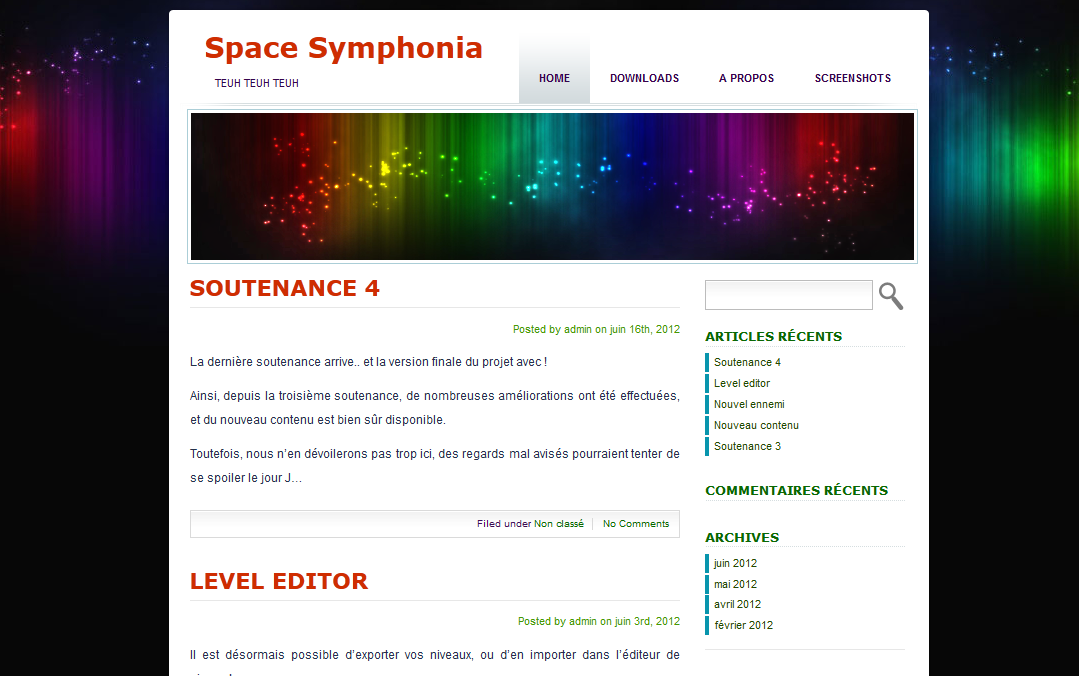
\includegraphics[width=9cm]{images/site1.png}
\end{center}

\par Nous avons peu à peu rajouté une section « Téléchargements » où il est possible de récupérer les sources, l'exécutable et l'installateur : 

\begin{center}
	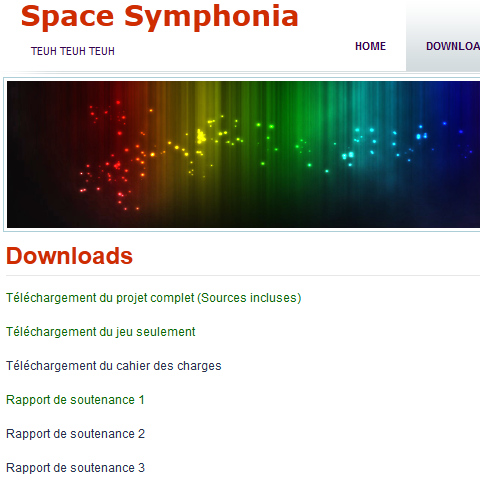
\includegraphics[width=9cm]{images/site2.png}
\end{center}

Puis également une section « À propos » où vous pouvez trouver des informations de contact:

\begin{center}
	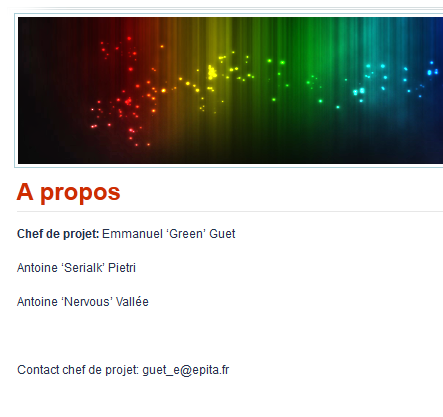
\includegraphics[width=9cm]{images/site3.png}
\end{center}

Et enfin une section « Screenshots » où l'on peut voir différentes captures d'écran qui montrent l'évolution de notre jeu :

\begin{center}
	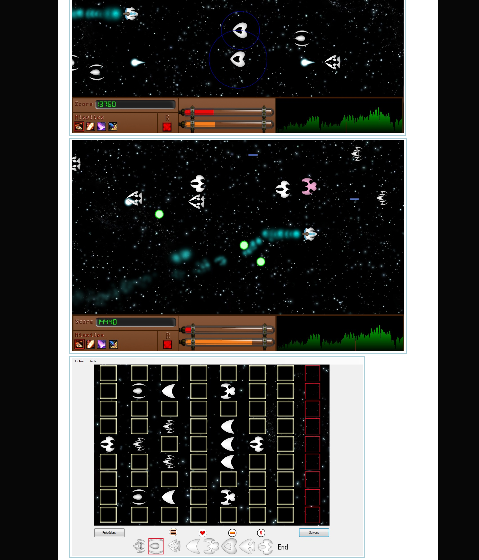
\includegraphics[width=9cm]{images/site4.png}
\end{center}

Le site est une installation Wordpress de base hébergée sur un VPS (Virtual Private Server) tournant sur une Debian Squeeze (avec php5 et lighttpd) administrée par Antoine Pietri. Nous avons acheté le domaine space-symphonia.fr et redirigé vers ce VPS, qui, via lighttpd, le route vers notre site.
		\subsection{Graphismes}
			\par Les membres du groupe responsables de cette partie étaient Antoine Vallée et Antoine Pietri.

\par Depuis la seconde soutenance, nous faisons progresser un site web en lui ajoutant au fur et à mesure du contenu.
Nous avons depuis le début une page de news que nous mettons régulièrement à jour :

\begin{center}
	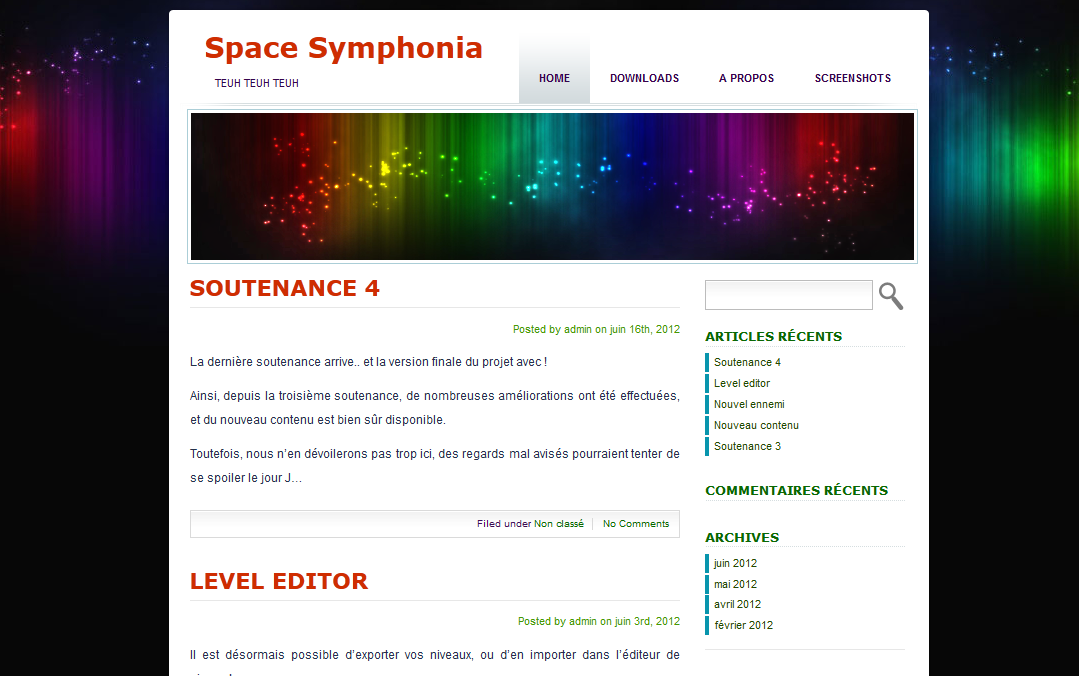
\includegraphics[width=9cm]{images/site1.png}
\end{center}

\par Nous avons peu à peu rajouté une section « Téléchargements » où il est possible de récupérer les sources, l'exécutable et l'installateur : 

\begin{center}
	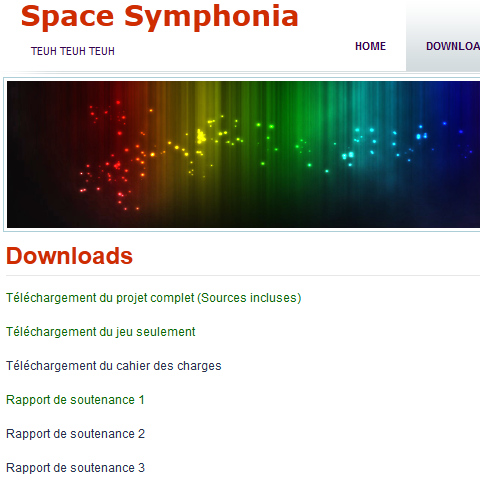
\includegraphics[width=9cm]{images/site2.png}
\end{center}

Puis également une section « À propos » où vous pouvez trouver des informations de contact:

\begin{center}
	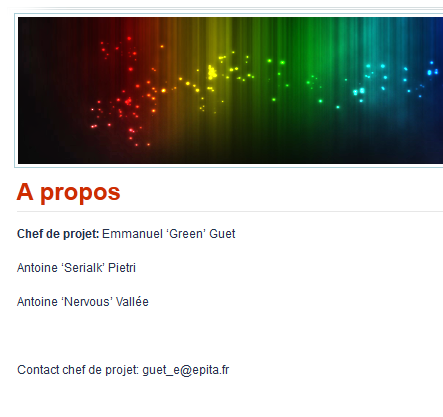
\includegraphics[width=9cm]{images/site3.png}
\end{center}

Et enfin une section « Screenshots » où l'on peut voir différentes captures d'écran qui montrent l'évolution de notre jeu :

\begin{center}
	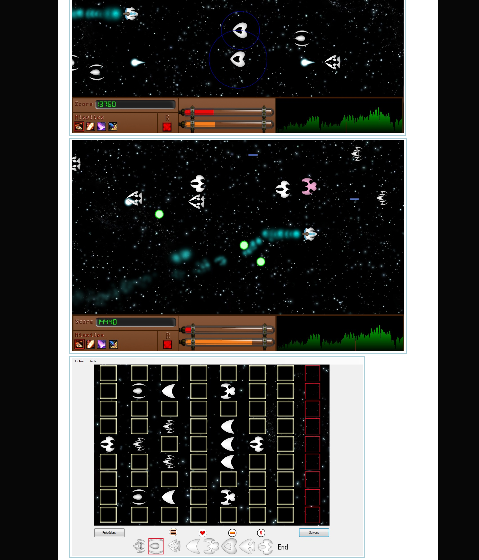
\includegraphics[width=9cm]{images/site4.png}
\end{center}

Le site est une installation Wordpress de base hébergée sur un VPS (Virtual Private Server) tournant sur une Debian Squeeze (avec php5 et lighttpd) administrée par Antoine Pietri. Nous avons acheté le domaine space-symphonia.fr et redirigé vers ce VPS, qui, via lighttpd, le route vers notre site.
	
	\section{Récit du déroulement du projet}
		\par La réalisation de ce projet ne s'est pas faite sans mal. Il y a bien sûr eu des moments difficiles et des moments de frustration. Chercher à comprendre un problème dans un menu la veille d'une soutenance tard dans la nuit n'est pas aussi amusant que ce à quoi on pourrait s'attendre. Nous avons du également gérer les tensions au sein du groupe pour aller vers l'avant quels que soient les problèmes rencontrés.
\par Réaliser ce projet a tout de même été un enrichissement personnel pour nous tous, et nous a rendu plus forts\footnote{Ce projet ne nous a pas tué, ce qui ne nous tue pas nous rend plus fort, donc ce projet nous a rendu plus forts}. Certaines étapes de sa réalisation ont parfois entraîné une grande fierté, que ce soit pour une simple correction après avoir passé des heures à comprendre le problème, ou à l'opposé voir son algorithme d'analyse sonore marcher est un sentiment merveilleux.
\par De plus, le jeu final correspond parfaitement à nos attentes. Nous ne nous attendions pas, au début de l'année, à parvenir à un jeu aussi abouti, diversifié et détaillé. Nous avons ajouté plus de contenu que prévu, et le mode libre est un grand succès, si bien que nous avons parfois envie de jouer à notre propre jeu.	
			
	\section{Résultat final par rapport à nos attentes}
		\input{parties/resultat-final}
	
	\section{Conclusion}
		\par En conclusion, ce projet dépasse la hauteur de nos espérances et il a été pour nous tous un grand enrichissement personnel. Gérer les tensions nous en a appris beaucoup sur la gestion d'un projet et la fierté de voir un projet de cette ampleur abouti est inégalable.
		\par Nous espérons continuer dans cette lignée au cours des 4 prochaines années qui nous séparent du diplôme d'ingénieur, et espérons reproduire cette expérience formidable qu'a été le développement d'un jeu vidéo.
		\vspace{2cm}		
		\par \emph{We will sing to you, Doctor. The universe will sing you to your sleep. This song is ending. But the story never ends.}
\end{document}
